\section{Experiments}
\label{sec:experiment}
In this section, we first present dataset and evaluation metrics used in our experiments. Then we explore and evaluate several design choices of our framework 
and compare their effectiveness against previous methods.

\subsection{Dataset}
\label{sec:data}
Our MCQ dataset covers multiple domains including science,  
vocabulary, common sense and trivia.
It is compiled from a wide variety of open source  
MCQ dataset including SciQ~\cite{welbl2017crowdsourcing}, 
MCQL~\cite{liang2018distractor}, AI2 Science Questions, 
AI2 4th Grade Science Exams as well as trivia, and 
vocabulary MCQs crawled from websites. 
We filter out MCQs whose keys are not short phrases since this paper only 
focuses on extractive cloze-style DG, 
which results in 2,880 items in total. 
Table \ref{table:dataset} summarizes the statistics of our dataset. The part-of-speech (POS) distributions of the keys are also presented in \figref{fig:pos}.

\begin{table}[thb!]
\small
\addtolength{\tabcolsep}{-2pt}
\centering
	\begin{tabular}{l|c|cccc}
		\toprule
		\multirow{2}{*}{Domain} & \multirow{2}{*}{Total} & \multirow{2}{*}{Science} & \multirow{2}{*}{Vocab.} & \multirow{2}{*}{\shortstack{Common\\Sense}} & \multirow{2}{*}{Trivia}\\
		& & & & & \\
		\midrule
		\# MCQs & 2880 & 758 & 956 & 706 & 460\\
		\midrule
		\# Distractors & 3.13 & 3.00 & 3.99 & 3.48 & 2.99\\
		\bottomrule
	\end{tabular}
	\caption{Dataset Statistics (number of MCQs in each domain and average number of distractors per question)}
	\label{table:dataset}
\end{table}
\begin{figure}[htb!]
	\centering
	\scalebox{1.0}{\includegraphics[width=1.0\columnwidth]{figure/dist.eps}}
	\caption{Part-of-speech distribution of keys in different domains.} \label{fig:pos}
\end{figure}
We convert questions to cloze form by constructing Penn Treebank style trees using Stanford Parser~\cite{klein2003accurate}, and adjusting node order according to the identified question type. For the following experiments, the dataset is randomly devided into train/valid/test with an approximate ratio of 8:1:1.
We use the tokenizer and POS tagger from NLTK~\cite{Loper:2002:NNL:1118108.1118117} to preprocess the stems and keys when constructing features.
\subsection{Evaluation Metrics}
\label{sec:metrics}
% We use the following metrics to evaluate distractor generation methods:

~~\textbf{Human Annotation} Following~\citet{jiang2017distractor}, we ask three proficient English speakers to evaluate distractors' reliability and plausibility without showing them the key. We evenly sample 50 items in all domains from test set, each item contains multiple distractors including 3 generated by each method and all ground truth distractors 
designed by human experts. For each distractor, the judges decided whether 
it is correct or incorrect given the context. For a distractor deemed to 
be incorrect, the reliability score is 1 and the judges further assess 
its plausibility on a 3-point scale: 
``Obviously Wrong'' (0 point), 
``Somewhat Plausible'' (1 point), 
or ``Plausible'' (2 points).  
% 从 human evalution 结果来看,很多ground truth也不是 good distractor.我们的framework 只能尽可能的接近ground truth 的质量,所以有时候不合理

\textbf{Ranking Measures} 
% To some extent, whether the ground truth distractors 
% come out on the top of the result list demonstrate the effectiveness of 
% the distractor generator. 
Following~\citet{liang2018distractor}, we report top F1 score(F1@3), 
precision(P@1, P@3) and recall~(R@3) to show how well the generated distractors 
match the ground truth distractors, 
as well as the mean reciprocal rank (MRR) and normalized discounted 
cumulative gain (NDCG@10) to show the positions of ground truth distractors 
in the output ranked list. 
% Intuitively, we consider the ground truth distractors designed by human experts as good distractors.  

\textbf{Semantic Similarity} Sometimes the generated distractors
do not exactly match the ground truth, but are semantically very close. 
Word2vec~\cite{mikolov2013distributed} model trained on Wikipedia dump 
is utilized to measure the averaged maximum semantic similarity~(Semantic Similarity@3) between top three generated 
distractors and ground truth distractors. 

\subsection{Design Choices of CSG and DS}
\label{sec:ablation}



% \begin{table*}[th]
% \small
% \centering
% 	\begin{tabular}{|l|c|c|c|c|c|}
% 		\hline
% 		Method & P@1(\%) & P@3(\%) & MRR(\%) & NDCG(\%) & Semantic Similarity\\
% 		\hline
% 		CSG+DS & \textbf{10.42} & \textbf{6.17}  & \textbf{18.24} & \textbf{19.35} & \textbf{0.310}\\
% 		\hline
% 		--~Contextual Sim & 3.06 & 1.96 & 5.58 & 6.60 & 0.121\\
% 		\hline
% 		--~Web-search Score & 5.63 & 4.41 & 10.25 & 1.83 & 0.204\\ 
% 		\hline
% 		--~both & \textbf{7.76} & \textbf{5.91} & \textbf{12.85} & \textbf{13.41} & \textbf{0.214}\\
% 		\hline
% 	\end{tabular}
% 	\caption{Ablation over reliability-related features. }
% 	\label{table:ex1}
% \end{table*}

% \begin{table*}[th]
% 	\small
% 	\centering
% 	\begin{tabular}{|l|c|c|c|c|c|}
% 		\hline
% 		Method & P@1(\%) & P@3(\%)  & MRR(\%) & NDCG(\%) & Semantic Similarity\\
% 		\hline
% 		CSG+DS & \textbf{10.42} & \textbf{6.17}  & \textbf{18.24} & \textbf{19.35} & \textbf{0.310}\\
% 		\hline
% 		--~second stage ranker & 5.79 & 4.24 & 11.34 & 14.02 & 0.270\\
% 		\hline
% 		--~first stage ranker & 7.33 & 4.50  & 12.49 & 13.41 & 0.239\\
% 		\hline
% 		--~both & 7.33 & 4.50 & 12.49 & 13.41 & 0.239\\
% 		\hline
% 	\end{tabular}
% 	\caption{Ablation over ranker. --both means we only use our candidate set generator(CSG) described in \secref{sec:CSG}}
% 	\label{table:metrics}
% \end{table*}

% We experiment with a wide variety of instantiations of CSG and DS which we consider to be representative.
% We conduct feature ablation on our ranker to examine the effectiveness of reliability checking feature, as well as ablation on 
% ranking model to probe the usefulness of cascaded learning strategy and list-wise ranking objective.
% \subsection{Effect of Using Different Distractor Selectors}
% To illustrate the effectiveness of our distractor selector, we compare it with several baseline methods by running with the Probase candidate set generator separately:

% \textbf{-Reliability Checking (-RC)} is a naive version of our distractor selector. It excludes LM score and Web-search score from the distractor selector.
% \subsubsection*{Instantiation of CSG}
We investigate Probase and WordNet as the knowledge base in CSG and additionally extract all words and phrases from WordNet as a baseline of CSG in following experiments. For Probase, both $p(c|a)$ and $p(d|c)$ are natively supported and can be obtained using official APIs. Size of concept set $C$ is set to be 20. For nouns and verbs in WordNet, we treat the set of unique hypernyms~(as well as their siblings) of all synsets for $a$ as concept set $C$ and compute
$p(c|a)$ using the Laplace-smoothed Bayes rule on the lemma frequency provided in WordNet~(count on sense tagged text). We choose all synsets and their similar/antonymic sets as concept set $C$ for adjectives and adverbs in WordNet. Topic distributions $\pi_{a,q}$ and $\gamma_c$ are obtained using LDA pre-trained on Wikipedia dump and $K$ is set to 100.

% \subsubsection*{Instantiation of DS}
% As mentioned before in \secref{sec:DS}, one can customize DS with various learning-to-rank model. 
For DS, we experiment with point-wise, pair-wise and list-wise ranking models to find the best practice.
Specifically, we employ AdaBoost~\cite{freund1997decision} as point-wise ranker and LambdaMART~\cite{burges2010from} as both pair-wise and list-wise ranker due to their fine performance. For the training of DS, negative examples are sampled using top 100 candidates extracted by CSG excluding those that are within ground truths. At test time, DS takes as input 30 candidates extracted by CSG 
and 20,000 candidates sampled from WordNet's own vocabulary.

% Evaluation results of different instantiations are presented in \secref{sec:res}.
% \textbf{Probase Probability} yields candidates belonging to the same concept as the key and ranks them directly according to statistical probability stored in Probase. 

% \textbf{Candidate Filtering (CF)} excludes all the candidates that appear in the web search result of the stem~\cite{sumita2005measuring}. 


% \XZ{to be implemented}
% \textbf{Hit Score} replace our correctness score with hit score \XZ{to be implemented}

% As shown in Table \ref{table:metrics}, our method and its naive version -RC achieves much better perfomance than the two methods. Reasonably, -RC performs better in terms of NDCG and semantic similarity as it excludes reliability checking features that, to some extent, help ``filter'' correct answers from the final n-bast distractor list. e.g. For the stem ``\textit{is considered a good source of calcium}'' and the key \textit{milk}, -RC generates \textit{kefir}, a correct answer, as the best distractor. On the other hand, \textit{kefir} is not contained in the 10-best distractor list generated by our method, but \textit{kefir} have higher semantic similarity than other candidates.     
\subsection{Baselines}
We name our framework \textbf{CSG+DS} and compare it against the following baselines:
\begin{itemize}
	\item \textit{Thesaurus-based Method (TM)}~\cite{sumita2005measuring} ranks candidate distractors from synonyms of the key in WordNet based on path similarity and filters out those that appear in the documents retrieved from the Web. 
	\item \textit{RevUP}~\cite{Kumar2015RevUP} ranks candidate distractors based on weighted average of word2vec similarity, dice coefficient and language model probability.
	\item \textit{EmbSim+CF}~\cite{jiang2017distractor} combines word2vec similarity and tri-gram/dependency in ranking and filtering respectively.
	\item \textit{ED} calculate the Levenshtein edit distance to measure the spelling similarity between distractors and key.
	\item \textit{BERT}~\cite{devlin2018bert} ranks candidates based on cosine similarity of their BERT embeddings with that of the key.
	\item \textit{LR+RF}~\cite{liang2018distractor} combines logistic regression and random forest as a two-stage cascaded ranker with features measuring the plausibility of distractors.
	\item \textit{LR+LM}~\cite{liang2018distractor} replaces random forest in LR+RF with LambdaMART.
	% \item \textit{BERT}~\cite{devlin2018bert} predicts blank gap in the stem as distractors based on contextual information.
\end{itemize}
Trigram and 5-gram Kneser Ney language model are built upon the original corpus of our dataset. Word2Vec~(CBOW) is pre-trained on Wikipedia dump and fine-tuned on our corpus. Dependency parsing tree is obtained using Spacy toolkit~\cite{spacy2}. We fetch the uncased, base version of BERT~\cite{Wolf2019HuggingFacesTS} and fine-tune it on our corpus.

% For both Word2Vec and Word2Vec+Reranking we use CBOW model trained on English Wikipedia dump. For BERT and BERT+Reranking, we use the base, uncased BERT model pretrained on BooksCorpus and English Wikipedia. LR+RF's candidate set include all keys and distractors from the dataset it is trained on and is evaluated using the same scikit-learn~\cite{scikit-learn} library and features described in the original paper~\cite{liang2018distractor}. 

% In this part, we will show the performance of different methods on 
% our newly-constructed dataset and provide some analysis. 
%\KZ{Make the examples below in one separate line so that they stand out?} 
\subsection{Results \& Analysis}
\label{sec:res}
% The overall results on test set are shown in Table \ref{table:human}. 
% We empirically observe that our CSG+DS method outperforms all unsupervised baselines and previous state-of-the-art learning-based model in terms of plausibility and reliability as well as various ranking measures by a large margin.
\subsubsection*{Combinations of CSG and DS}
\begin{table*}[th]
	\small
	\centering
	\begin{tabular}{cc c c c c c c c}
		\toprule
		\multicolumn{2}{c}{\textbf{Instantiation}} &\multirow{2}{*}{F1@3} &\multirow{2}{*}{P@1} &\multirow{2}{*}{P@3} &\multirow{2}{*}{R@3} &\multirow{2}{*}{MRR} &\multirow{2}{*}{NDCG@10} &\multirow{2}{*}{\tabincell{c}{Semantic \\Similarity@3}} \\
		\\ [-1.8ex]
		\cline{1-2}
		\\ [-1.8ex]
		CSG &DS & & & & & & &\\
		\midrule
		\multirow{4}{*}{WordNet} &- &3.14 &3.49 &2.33 &5.43 &7.19 &8.66 &27.55 \\
		&point-wise ranker &7.26 &9.30 &5.55 &11.95 &14.30 &14.63 &36.50 \\
		&pair-wise ranker &7.11 &\textbf{10.07} &5.30 &12.14  &\textbf{14.40} &14.84 &35.35 \\
		&list-wise ranker &\textbf{7.71} &9.31 &\textbf{5.81} &\textbf{12.98} &14.34 &\textbf{14.94} &\textbf{36.68} \\
		\midrule
		\multirow{4}{*}{Probase} &- &5.88 &6.98 &4.39 &9.95  &12.07 &13.40 &35.44 \\
		&point-wise ranker &7.91 &8.14 &5.94 &12.98  &15.09 &17.69 &41.39 \\	
		&pair-wise ranker &\textbf{9.42} &10.08 &\textbf{7.00} &15.88  &17.33 &\textbf{19.70} &40.31 \\
		&list-wise ranker &9.19 &\textbf{10.85} &6.72 &\textbf{15.88}  &\textbf{17.51} &19.31 &\textbf{41.71} \\
		\midrule
		\multirow{4}{*}{w/o CSG} &- &- &- &- &- &- &- &- \\
		&point-wise ranker &5.59 &4.63 &3.98 &10.29 &8.67 &11.02 &36.21 \\
		&pair-wise ranker &5.62 &\textbf{5.01} &3.98 &10.10  &\textbf{9.28} &\textbf{11.60} &\textbf{36.51} \\
		&list-wise ranker &\textbf{5.94} &4.24 &\textbf{4.24} &\textbf{10.81} &8.81 &11.46 &35.93 \\
		\bottomrule
	\end{tabular}
	\caption{Comparison of combinations of different choices of CSG and DS. - means there is no ranking algorithm to be evaluated.}
	\label{table:instantiations}
\end{table*}
% Most baselines we compare to are built upon various knowledge base or fixed vocabulary(denoted in the legend).~Hence, we first examine the capacity of different candidate sources by calculating the recall without re-ranking step\footnote{Candidate filtering in TM, word2vec similarity in WP and BERT+WS.}.~\tabref{table:recall} summarizes the average Recall@K of CSG, BERT\footnote{BERT+WS without re-ranking is identital to BERT and is omitted here.}, WP and TM. Our sole CSG achieve significantly higher recall than the others~(see \figref{fig:recallk} for results on different domains), indicating larger capacity for DG task. Note that we do not compare with Recall@K of LR+RF since it use all the keys and distractors in dataset as candidate set which naturally leads to high recall.
% \figref{fig:recallk} shows the Recall@1500 of Probase CSG and WordNet CSG in all domains. 
% Probase CSG achieves much higher recall than WordNet CSG in all domains except for vocabulary, which well aligns with the fact that Probase possesses much larger coverage over real-world entities yet suffers from sparsity of verbs and adjectives.

\tabref{table:instantiations} shows the automatic evaluation results for different combinations of CSG and DS. Without CSG, distractor selector trained with trivial negative examples is forced to select distractors from a rather large and noisy candidate set therefore the performance is clearly worse. 
We also find that combining CSG with DS yields consistent improvement 
by all metrics and the improvement is more significant for WordNet CSG, 
which is mainly because $p(c|a)$ and $p(d|c)$ in WordNet are partly biased 
due to the limited scale of corpus they are estimated on, hence the 
supervised training will lead to more performance gain. Pair/list-wise ranker achieve comparable performance mainly due to the binarized relevance score.
Since named entities and common nouns mainly underpin Probase, 
DS with Probase CSG naturally get higher ranking scores on our dataset 
than its counterpart with WordNet CSG.

\begin{table*}[th]
	\small
	\centering
		\begin{tabular}{lc cc c c c c c cc}
			\toprule
			\multirow{3}{*}{\textbf{Method}} &\multicolumn{2}{c|}{\textbf{Human Evaluation}} &\multicolumn{7}{c}{\textbf{Automatic Evaluation(\%)}} \\
			\\ [-1.8ex]
			\cline{2-10}
			\\ [-1.8ex]
			& Reliability & Plausibility  &F1@3 & P@1 & P@3 &R@3 & MRR & NDCG@10 & \tabincell{c}{Semantic \\ Similarity@3}\\
			\midrule
			TM &95.57\%  &1.25$\pm$0.41 &1.74 &0.40  &1.16  &3.48   &2.69  &4.79  &21.91 \\
			\midrule
			\textbf{WordNet CSG} &98.66\% &1.25$\pm$0.34 &3.14 &3.49 &2.33 &5.43 &7.19 &8.66 &26.55 \\
			+~ED &98.66\% &1.26$\pm$0.41  &0.41 &0.12  &0.26  &0.58  &2.10  &1.93  &20.92 \\
			+~RevUP &98.65\%  &1.22$\pm$0.34  &4.07 &5.79  &3.21  &6.43 &9.31  &9.60  &32.09 \\
			+~EmbSim+CF &\textbf{99.12}\%  &1.21$\pm$0.49  &4.62  &6.17  &3.60  &7.40  &10.32  &10.94  &36.52 \\
			+~BERT &91.94\% &1.23$\pm$0.58  &5.68 &6.93  &4.23  &9.57  &11.10  &11.66  &30.78 \\
			+~LR+LM &98.66\%  &1.25$\pm$0.35 &6.48 &9.25  &4.89 &10.81   &13.42 &13.66 &29.11\\
			+~LR+RF &98.56\%  &1.25$\pm$0.38 &6.67 &8.10 &5.14 &10.81   &13.18 &13.73 &30.46 \\
			+~\textbf{DS(lise-wise)} &98.66\%  &\textbf{1.35$\pm$0.40}   &\textbf{7.71} &\textbf{9.31} &\textbf{5.81} &\textbf{12.98} &\textbf{14.34} &\textbf{14.94} &\textbf{36.68} \\
			\midrule
			\textbf{Probase CSG} &99.23\% &1.26$\pm$0.35 &5.88 &6.98 &4.39 &9.95  &12.07 &13.40 &34.44 \\
			+~ED &98.33\%  &1.23$\pm$0.38  &0.82 &1.16  &0.65  &1.30  &5.02  &4.92  &28.38 \\
			+~RevUP &98.87\%  &1.26$\pm$0.36  &6.27 &5.40  &4.63  &10.68  &11.74  &14.23  &37.11 \\
			+~EmbSim+CF &98.98\%  &1.19$\pm$0.47  &7.01 &8.10  &5.14  &12.34  &13.86  &16.33  &41.26 \\
			+~BERT &98.00\% &1.27$\pm$0.58  &7.05 &7.72  &5.14  &12.23  &13.60  &16.21  &36.30 \\
			+~LR+LM &98.98\%  &1.25$\pm$0.30   &7.62  &8.53  &5.81 &12.27 &15.56 &16.83 &40.18 \\
			+~LR+RF &99.13\%  &1.24$\pm$0.31   &7.48 &8.52 &5.42 &13.17   &15.87 &19.03 &40.72\\
			+~\textbf{DS(list-wise)} &\textbf{99.33}\%  &\textbf{1.30$\pm$0.34} &\textbf{9.19}  &\textbf{10.85} &\textbf{6.72} &\textbf{15.88} &\textbf{17.51} &\textbf{19.31} &\textbf{41.71} \\
			\midrule
			\textbf{w/o CSG} &- &- &- &- &- &-  &- &- &- \\
			+~ED &\textbf{99.98}\%  &1.00$\pm$0.12  &0.19 &0.38  &0.12  &0.38  &0.54  &0.53  &11.22 \\
			+~RevUP &98.88\%  &1.02$\pm$0.14  &2.01 &2.35  &1.35  &4.21  &3.95  &5.12  &38.89 \\
			+~EmbSim+CF &97.77\%  &0.93$\pm$0.52  &2.12 &2.70  &1.41  &4.24  &4.19  &5.24  &\textbf{42.78} \\
			+~BERT &98.87\% &1.02$\pm$0.24  &3.03 &2.88  &2.15  &5.14  &5.29  &6.78  &39.89 \\
			+~LR+LM &97.77\%  &1.05$\pm$0.28   &4.22  &4.34  &2.79 &8.69 &7.02 &10.16 &41.60 \\
			+~LR+RF &97.78\%  &1.02$\pm$0.20   &4.05  &4.21 &2.66 &8.55 &6.91 &10.08 &40.29\\
			+~\textbf{DS(pair-wise)} &99.43\%  &\textbf{1.06$\pm$0.14} &\textbf{5.59} &\textbf{5.01} &\textbf{3.98} &\textbf{10.10}  &\textbf{9.28} &\textbf{11.60} &36.51\\
			\midrule
			ground truth &\textbf{100\%}  &\textbf{1.41$\pm$0.35}  & - & - & - & - & - & - & -\\
			\bottomrule
		\end{tabular}
		\caption{End-to-end comparison on test set. - means no ranking algorithm to evaluate and ``ground truth'' denotes the score of ground-truth distractors associated with each item. The \textit{kappa} inter-annotator agreement is 0.44.}
		\label{table:human}
	\end{table*}
% \begin{figure}[htb]
% 	\centering
% 	\scalebox{1.0}{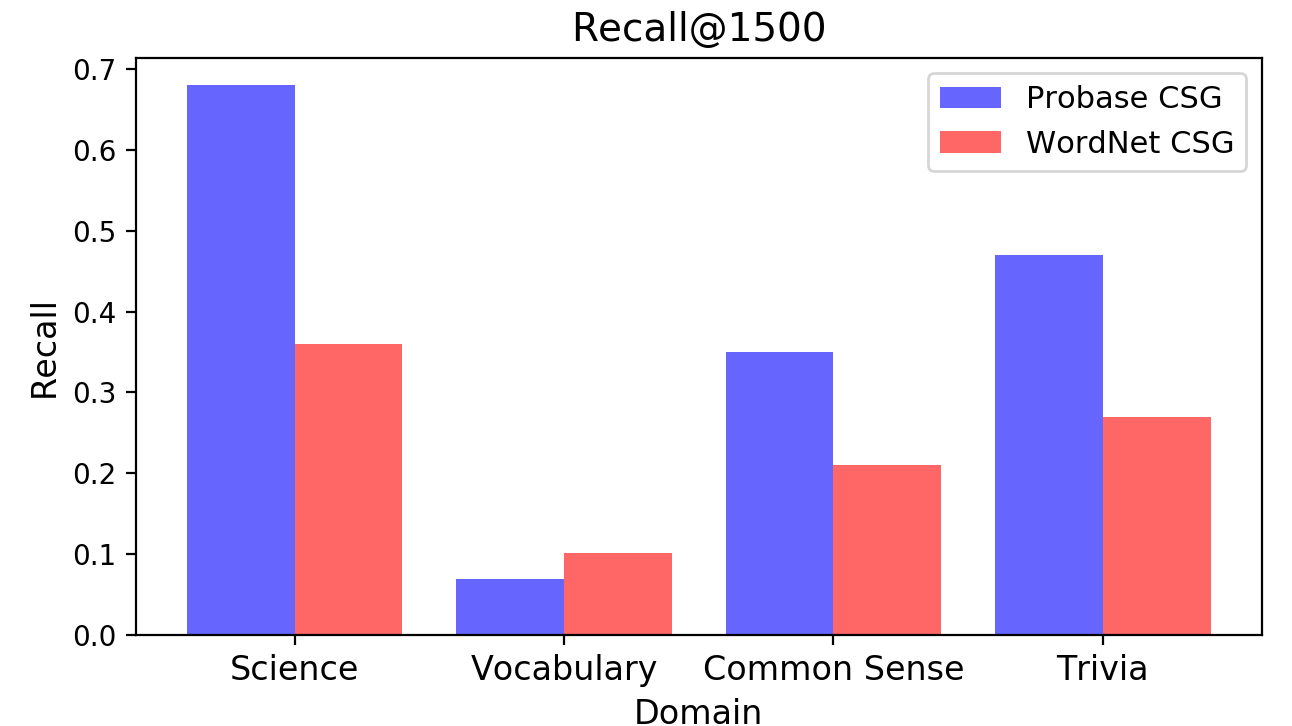
\includegraphics[width=1.0\columnwidth]{figure/recall.png}}
% 	\caption{Recall@1500 of Probase CSG and WordNet CSG in different domains.} \label{fig:recallk}
% \end{figure}

% \begin{table}[htb!]
% 	\small
% 	\centering
% 	\begin{tabular}{|c|c|c|c|c|}
% 		\hline
% 		K &  50 & 500 & 1000 &  1500 \\
% 		\hline
% 		WordNet CSG & 11.9\% & 23.5\% & 25.7\% & 26.5\%\\
% 		\hline
% 		Probase CSG & \textbf{22.8}\% & \textbf{39.3}\% & \textbf{45.1}\% & \textbf{47.8}\%\\
% 		\hline
% 	\end{tabular}
% 	\caption{Recall@K of WordNet CSG and Probase CSG without DS. Results are averaged across all domains.}
% 	\label{table:recall}
% \end{table}
\subsubsection*{Domain Analysis}
\begin{figure}[hb!]
	\centering
	\subfigure[F1@3 score in different domains.]{
	\begin{minipage}[b]{0.5\textwidth}
	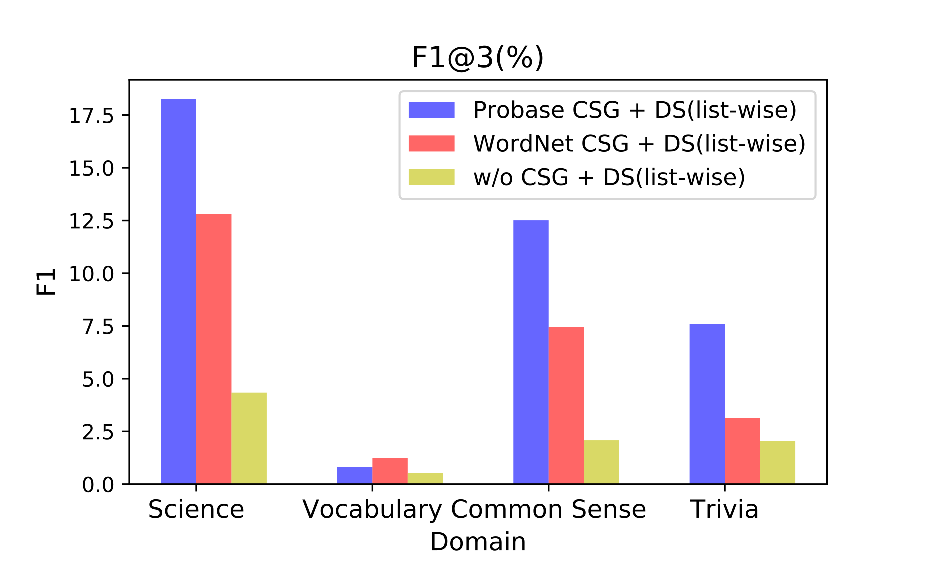
\includegraphics[width=1\columnwidth]{figure/f1.eps}
	\end{minipage}
	}
	\subfigure[NDCG@10 score in different domains.]{
	\begin{minipage}[b]{0.5\textwidth}
	\includegraphics[width=1\columnwidth]{figure/ndcg.eps}
	\end{minipage}
	}
	 \caption{F1@3 and NDCG@10 in different domains.} \label{fig:domains}
\end{figure}

\figref{fig:domains} shows the F1@3 and NDCG@10 in different domains. All three methods show the same trend when evaluated in different domains. The performance drops most drastically when applied in vocabulary domain because adjectives and adverbs in Probase and WordNet are either rare or not hierarchically organized. Another possible explanation is that the ground truth distractors in vocabulary domain are less semantically-related to the key than those in other domains, which makes learning process of the ranker oscillatory .

Our framework is especially better at generating distractors in the domain of science and common sense, in which the keys and ground-truth distractors are mostly subject-specific~(e.g. physics) terminologies, real-world entities and other common nouns. Trivia domain has similar characteristic but the keys are often rarer, therefore Probase suffers less due to its larger scope.
\subsubsection*{End-to-End Comparison} 
\label{sec:endtoend}
\tabref{table:human} shows the results by running aforementioned baselines and DS with or without CSG.

Despite the significantly reduced number of candidates, ranking methods with our candidate set generator can achieve much higher performance than with unstructured vocabulary in much shorter runtime. TM performs badly due to its naive path similarity ranking criterion. The results of ED are worst among all unsupervised methods while embedding based methods can even achieve comparable performance against LR+LM/RF when provided with a high-quality candidate set.
BERT ranks distractors using contextualized representation thus leading to lowest reliability according to human evaluation. 
LR+RF/LM achieves similar ranking performance yet obtain poorer reliability than CSG+DS since they only focus on the plausibility of selected distractors. CSG+DS, despite its relative simplicity, obtain consistent improvements over LR+RF/LM without two-stage cascaded training.

We also found that automatic evaluation and human-annotation of
the plausibilities for the baselines are not necessarily 
positively correlated, part of the reason may be that methods such as LR+RF/LM focus much on shallow feature patterns of ground-truth distractors and fail to unearth potential acceptable distractors.
However, distractors generated by CSG+DS yield highest ranking measures while rated as most plausible by human annotators. 
Unsupervised methods work solely relying on the semantic similarity hence their reliabilities are generally lower than supervised ones. EmbSim+CF gets higher reliability with WordNet, whose unreliable candidates get more chance to be eliminated by post-filtering than those in Probase.
% Distractors generated by CSG+DS have very competitive quality, scoring on average 1.12, even higher than the average score of the ground truth designed by human experts. They are also less likely to be rated ``Obviously Wrong.'' 
% The reason is that, different from other methods, 
% CSG+DS method can make full use of the rich information in the stem 
% to generate distractors belonging to the same concept-level as the key 
% with contextual fit, which is also challenging for human experts. 
% For example, for the stem ``\textit{\underline{\hbox to 8mm{}} functions primarily to defend the body against disease.}'' and the key ``\textit{immune}'', our CSG+DS method generates ``\textit{reproductive, respiratory, digestive}'' which belong to the same concept \textit{functions} as the key. On the other hand, the ground truth distractor \textit{nervous} is not similar to the key enough. TM and WP achieve low plausibility since it does not consider latent context, leading to many obviously wrong distractors. Although WP does make use of context words, it treats the key and other context words similarly and may select distractors similar to a context word instead of the key.  

% CSG+DS shows a significant improvement in reliability compared with baselines. TM, with 83.96\% reliability, is more prone to yield invalid distractors that are correct answers. This is not unexpected since it tries to find distractors from synonyms of the key, which are likely to have exactly the same meaning as the key.
% However, CSG+DS retrieves candidates belonging to the same concept-level, thus generate less invalid distractors. We also find that, with the same CSG, adding DS component helps improve the reliability rate, which verifies the effectiveness of our reliability checking features.
% {Case Study \& Discussion}

% \begin{table*}[htb!]
% 	\small
% 	\centering
% 		\begin{tabular}{|l|c c c c c c c |c|}
% 			\hline
% 			\multirow{3}{*}{Method} &\multicolumn{7}{|c|}{Automatic Evaluation(\%)} \\
% 			\cline{2-8}
% 			&F1@3 & P@1 & P@3 &R@3 & MRR & NDCG@10 & \tabincell{c}{Semantic \\ Similarity@3}\\
% 			\hline
% 			\textbf{WordNet Vocab} &- &- &- &-  &- &- &- \\
% 			+~RevUP  &0 &0  &0  &0  &0  &  & \\
% 			+~EmbSim+CF  & &  &  &  &  &  & \\
% 			+~ED & &  &  &  &  &  & \\
% 			+~BERT & &  &  &  &  &  & \\
% 			+~LR+LM &  &  & & & & & \\
% 			+~LR+RF & & & &   & & &\\
% 			+~\textbf{DS(list-wise)} &\textbf{}  &\textbf{} &\textbf{} &\textbf{} &\textbf{} &\textbf{} &\textbf{} \\
% 			\hline
% 		\end{tabular}
% 		\caption{Results by replacing CSG with vocabulary extracted from WordNet.}
% 		\label{table:ablation}
% 	\end{table*}
\subsection{Case Study}
% \begin{table*}[ht!]
% 	\small
% 	\centering
% 		\begin{tabular}{|l|l|c c c c c c c|}
% 			\hline
% 			Method& Domain &F1@3 & P@1 & P@3 &R@3  & MRR & NDCG@10 & \tabincell{c}{Semantic \\Similarity@3}\\
% 			\hline
% 			\multirow{5}{*}{\tabincell{l}{WordNet CSG~+\\ list-wise ranker DS}} &Science &12.82  &21.73  &9.42 &21.73 &25.59 &23.29  &35.72 \\
% 			&Common Sense &7.45  &13.89  &5.56 &12.73 &15.80 &13.61 &27.45 \\
% 			&Vocabulary &0.43  &0.22  &0.28 &0.84  &0.72  &1.12  &24.18 \\
% 			&Trivia &3.13  &2.40  &2.61 &4.22 &7.61  &8.18  &24.99  \\
% 			\cline{2-9}
% 			&Total &7.71 &9.31 &5.81 &12.98 &14.34 &14.94 &34.68 \\
% 			\hline
% 			\multirow{5}{*}{\tabincell{l}{Probase CSG~+\\ list-wise ranker DS}} &Science &18.26  &28.26  &13.76 &30.43 &40.91  &38.35  &44.58 \\
% 			&Common Sense &12.51  &20.83  &10.19 &18.75 &27.28 &22.61 &33.47 \\
% 			&Vocabulary &0.41  &0.21  &0.27 &0.84  &0.58  &0.88  &12.75 \\
% 			&Trivia &7.59  &9.63  &6.42 &10.54 &20.39  &19.87  &34.49 \\
% 			\cline{2-9}
% 			&Total &9.19 &10.85 &6.72 &15.88 &17.51 &19.31 &40.71\\
% 			\hline
% 		\end{tabular}
% 		\caption{Results(\%) of the two best performing CSG+DS instantiations in different domains.}
% 		\label{table:domains}
% 	\end{table*}
\begin{table*}[htb!]%[th]
	\small
	\centering
		\begin{tabular}{lcccccccc} %/tabincell{c}{haha// heihei//zeze}
			\toprule
			\# &-  &RevUP &ED  & EmbSim+CF &BERT & LR+RF & LR+LM & \textbf{DS}\\
			\midrule
			1 &\color{red}protein   &\color{red}protein  &aldehydes  &starch &glycosaminoglycans  & hydrocarbon &methane    &\color{red} fat\\
			\midrule
			2 &alcohol  &alcohol  &carboxylic acid  &glycerol  &glycerol &methane  &\color{red}protein    &\color{red}protein \\
			\midrule
			3 &benzene  &amino acid  &alcohol   &\textbf{glucose}  &aldehydes &hormone  &hormone   &peptide \\
			% \hline
			% 4 &amino acid  &benzene  &protein  &pesticide  &pesticide   &hydrocarbon   &ethanol \\
			% \hline 
			% 5 &DNA  &DNA  &methane  &cardiovascular  &polysaccharides  &pesticide  &methanol \\
			\bottomrule
		\end{tabular}
		\caption{Top 3 distractors generated by different methods when running with Probase CSG(- denotes sole Probase CSG)
	given the stem ``The main source of energy for your body is \underline{\hbox to8mm{}}.'' and the key ``{\color{blue}carbohydrate}''. Red colored distractors are the ground truth, bold distractors are invalid distractors that are eligible to the stem.}
		\label{table:example}
	\end{table*}
\tabref{table:example} compares predictions made by all baselines and DS~(list-wise) when running with Probase CSG. We can see that Probase CSG alone and RevUP are both able to generate distractors belonging to the same concept level as the key and accurately match one ground truth. However, running Probase CSG with ED yields 
distractors that are more semantically distant from the key. 
Despite the use of candidate filtering, EmbSim+CF still produces candidates 
like ``glucose'', which is an eligible answer to the stem. 
BERT instead generate compound names that are too technical and belong to lower concept level than ground truth. 
Among all the supervised rankers, DS hits another ground-truth distractor 
``fat'' while LM+RF/LM predict some obviously wrong distractors 
such as ``methane'' due to its coarse-grained features.

We refer interested readers to supplementary material for more examples.

% We refer readers to supplementary metrial for more sample distractors generated by different methods.
